GRU (Gated Recurrent Unit) là một trong những kiến trúc mạng nơ-ron tái lặp (RNN) phổ biến được sử dụng. GRU giúp mô hình học cách xử lý và dự đoán các chuỗi dữ liệu thời gian một cách hiệu quả, bằng cách giải quyết các vấn đề như sự biến mất đạo hàm và khó khăn trong việc lưu trữ thông tin dài hạn. GRU bao gồm hai cổng chính: cổng cập nhật (update gate) và cổng khôi phục (reset gate). Cả hai cổng này giúp kiểm soát luồng thông tin trong mỗi bước thời gian của chuỗi đầu vào và quyết định xem thông tin nào sẽ được truyền tiếp và thông tin nào sẽ bị loại bỏ.

\begin{figure}[htbp]
\centerline{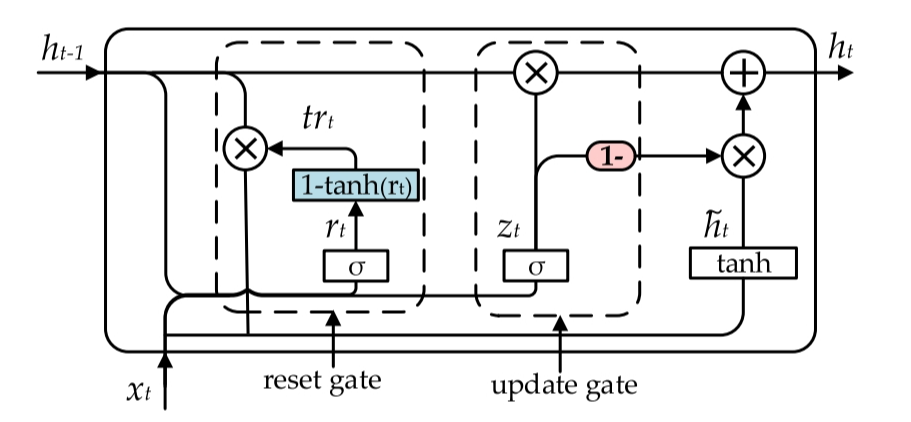
\includegraphics[width=0.4\textwidth]{img/GRU.png}}
\caption{Kiến trúc GRU}
\label{fig}
\end{figure}

Cổng Cập Nhật (Update Gate): Xác định mức độ thông tin mới sẽ được lưu trữ trong trạng thái ẩn mới (hidden state). Nó quyết định phần nào của trạng thái ẩn cũ nên được cập nhật bằng thông tin mới từ đầu vào hiện tại.

Cổng Khôi Phục (Reset Gate): Quyết định phần nào của trạng thái ẩn cũ sẽ được "quên" hoặc đặt lại. Nó xác định cách sử dụng thông tin từ các bước trước đó để tính toán trạng thái ẩn mới.

Sự kết hợp của hai cổng này cho phép GRU hiệu quả trong việc xử lý các chuỗi dài và giữ lại thông tin quan trọng trong quá trình huấn luyện.